\documentclass[11pt,a4paper]{article}
\usepackage[margin=2.5cm]{geometry}
\usepackage{amsmath,amssymb,booktabs,graphicx,xcolor,hyperref,microtype}
\usepackage{authblk}
\hypersetup{colorlinks=true,linkcolor=blue,citecolor=blue,urlcolor=blue}

\title{\textbf{Paper 55: Lyapunov Functional for VCML Identity Formation}\\
\large C\_order as a Regime-Local Monotone Scalar, and the
Noise-Floor Condition for Sustained Identity}

\author[1]{Gabriel Aubin-Moreau}
\affil[1]{Independent research}
\date{March 2026}

\begin{document}
\maketitle

\begin{abstract}
Paper~54 left two open questions about C\_order $= (D_\mathrm{nonadj} - D_\mathrm{adj})/\sigma_w$
as a candidate order parameter: (1)~Does C\_order have monotone positive drift toward
identity-encoding attractors (Lyapunov property)?
(2)~Can a single scalar organise all five behavioral axes?

We test C\_order over full formation trajectories across five behavioral regimes
(identity, parity, over-perturbed, patch, and C\_perturb noise-gated identity).

\textbf{Result:}
C\_order exhibits clear monotone positive drift
\emph{only} in the noise-gated regime (C\_perturb), rising from $\approx{-0.04}$ at
step~1000 to $\approx{+0.28}$ at step~2000 and plateauing near $+0.16$ at step~3000.
In all C\_ref conditions, $\sigma_w$ is $10{-}20\times$ larger, keeping C\_order near zero
or negative even when na\_ratio briefly exceeds~1 (transient identity).

\textbf{Key distinction:}
C\_order discriminates \emph{stable} identity (C\_perturb, sustained C\_order $>0$)
from \emph{transient} identity (C\_ref optimal, na $>1$ at step~2000 but
C\_order $< 0$ throughout).
The na\_ratio cannot make this distinction at any single timepoint.

\textbf{Analytical condition:}
C\_order has positive drift iff the signal growth rate exceeds the
noise growth rate: $\dot{D}_\mathrm{sig}/\sigma_w > C_\mathrm{order} \cdot \dot{\sigma}_w/\sigma_w$.
C\_perturb satisfies this by design ($\dot{\sigma}_w \approx 0$);
C\_ref violates it because $\dot{\sigma}_w > 0$ from writes to all quiescent cells.

\textbf{Theoretical implication:}
The Lyapunov property is not a universal feature of VCML dynamics (Paper~33 ruled
that out) but holds regime-locally in any condition that controls the noise floor.
The noise-gating mechanism (Paper~54) is the noise-floor condition for C\_order
to function as a Lyapunov scalar.
\end{abstract}

%──────────────────────────────────────────────────────────────────────────────
\section{Introduction}

\paragraph{Background.}
Paper~54 confirmed the correlation length law and showed that C\_perturb (write
trigger selectivity) maintains identity encoding at all perturbation amplitudes via
noise-gating: trigger selectivity reduces $\sigma_w$ (within-zone fieldM variance),
not the write-level information content.
Paper~54 proposed C\_order $= (D_\mathrm{nonadj} - D_\mathrm{adj})/\sigma_w$
as a candidate scalar that combines inter-zone contrast and noise floor.

\paragraph{The Lyapunov question.}
Paper~33 proved VCML is formally non-gradient (no $C^2$ Euclidean potential),
ruling out a global Lyapunov function for the full microscopic dynamics.
The question for Paper~55 is weaker and still informative:

\begin{quote}
\emph{Is there a coarse-grained scalar functional of fieldM with monotone
positive drift in the identity-forming adaptive regime?}
\end{quote}

A positive answer would unify the regime atlas: the quantity that the system
``climbs toward'' would organise the five control axes from Paper~53.
A negative answer would also be informative: it would mean the regime structure
is genuinely multi-scalar and cannot be compressed.

\paragraph{Structure of this paper.}
We test the Lyapunov property by tracking C\_order(t) over full trajectories
(3000 steps, 5 seeds) across five carefully chosen regimes spanning the
behavioral space.
We then derive the analytical condition under which C\_order has definite drift.

%──────────────────────────────────────────────────────────────────────────────
\section{Methods}

\paragraph{Regimes.}
All experiments use the S1 grid (W=80, H=40, zone\_width=10, WR=4.8).
Five regimes:

\begin{center}
\small
\begin{tabular}{llrrll}
\toprule
Regime & Write & supp & exc & r\_wave & Expected \\
\midrule
\texttt{ident\_opt}   & C\_ref     & 0.25 & 0.50 & 2 & Identity (standard optimal) \\
\texttt{parity\_sub}  & C\_ref     & 0.06 & 0.12 & 2 & Parity (amplitude below threshold) \\
\texttt{parity\_over} & C\_ref     & 0.80 & 1.60 & 2 & Parity (over-perturbed) \\
\texttt{patch}        & C\_ref     & 0.25 & 0.50 & 1 & Patch (corr.\ length failure) \\
\texttt{ident\_cp}    & C\_perturb & 0.06 & 0.12 & 2 & Identity (noise-gated) \\
\bottomrule
\end{tabular}
\end{center}

The \texttt{patch} regime uses r\_wave=1 at zone\_width=10 (ratio $= 10 > 5$),
violating the Paper~54 correlation length law.
The \texttt{ident\_cp} regime uses the same sub-threshold amplitude as
\texttt{parity\_sub} but with C\_perturb (write only during active wave events).

\paragraph{Tracking.}
Metrics recorded every 25 steps (120 timepoints per run).
Mean C\_order, na\_ratio, $\sigma_w$ computed over 5 seeds.

\paragraph{C\_order definition.}
With zone means $\bar{F}_z$ ($z=0,1,2,3$):
\begin{align}
D_\mathrm{adj}    &= \tfrac{1}{3}\sum_{|a-b|=1} \|\bar{F}_a - \bar{F}_b\| \\
D_\mathrm{nonadj} &= \tfrac{1}{3}\sum_{|a-b|>1} \|\bar{F}_a - \bar{F}_b\| \\
C_\mathrm{order}  &= (D_\mathrm{nonadj} - D_\mathrm{adj}) / \sigma_w
\end{align}
where $\sigma_w$ is the mean within-zone fieldM standard deviation.
C\_order $> 0$ iff non-adjacent zones are more separated in fieldM space than
adjacent zones --- the identity-encoding signature.

%──────────────────────────────────────────────────────────────────────────────
\section{Results}

\subsection{C\_order Trajectory by Regime}

\begin{table}[h!]
\centering
\small
\begin{tabular}{lrrrrl}
\toprule
Regime & C\_order(t=1000) & C\_order(t=2000) & C\_order(t=3000) & $\sigma_w$(t=2000) & na(t=2000) \\
\midrule
\texttt{ident\_cp}   & $+0.011$ & $+0.262$ & $+0.159$ & 0.012 & \textbf{1.493} [IDENTITY] \\
\texttt{ident\_opt}  & $-0.027$ & $-0.013$ & $-0.039$ & 0.202 & 1.026 [IDENTITY] \\
\texttt{parity\_sub} & $-0.007$ & $-0.010$ & $-0.026$ & 0.162 & 0.945 [parity] \\
\texttt{parity\_over}& $-0.022$ & $-0.007$ & $-0.036$ & 0.230 & 0.872 [parity] \\
\texttt{patch}       & $-0.014$ & $-0.019$ & $-0.007$ & 0.120 & 0.838 [parity] \\
\bottomrule
\end{tabular}
\caption{C\_order and related metrics at key timepoints across five regimes.
Only \texttt{ident\_cp} achieves sustained positive C\_order.
At step 2000, \texttt{ident\_opt} reaches na=1.026 (identity by na metric) but
C\_order remains negative ($-0.013$) because $\sigma_w = 0.202$ is too large.}
\end{table}

\textbf{Finding 1: Monotone positive drift in \texttt{ident\_cp} only.}
The C\_perturb condition is the \emph{only} regime where C\_order shows monotone
positive drift during the formation epoch (steps~1000--2000):
from $+0.011$ at step~1000 to $+0.262$ at step~2000 ($\Delta C_\mathrm{order} = +0.251$
over 1000 steps, mean drift $\approx +2.5 \times 10^{-4}$ per step).

After the formation peak (step~2000), C\_order decays slightly to a plateau
at $+0.159$ (step~3000), remaining positive throughout.
The post-peak decay reflects FIELD\_DECAY gradually erasing the formation signal,
balanced by ongoing wave-driven writing.

\textbf{Finding 2: Transient identity vs. stable identity.}
\texttt{ident\_opt} reaches na\_ratio~$= 1.026$ at step~2000
(matching Paper~54's measurement at STEPS=2000).
But C\_order at this same timepoint is $-0.013$: the system is formally in
identity by na\_ratio but C\_order is negative because
$\sigma_w = 0.202$ overwhelms the small positive
$(D_\mathrm{nonadj} - D_\mathrm{adj})$.

At step~3000, \texttt{ident\_opt} has retreated to na = 0.729 and
C\_order = $-0.039$.
The Paper~54 measurement at step~2000 captured the transient peak of a
non-sustained identity episode, not a stable attractor.

C\_order correctly identifies this distinction: \emph{negative} C\_order
even when na momentarily exceeds 1, flagging that the identity is not
supported by sufficient noise reduction to be self-sustaining.

\textbf{Finding 3: C\_ref parity and patch regimes are indistinguishable.}
\texttt{parity\_sub}, \texttt{parity\_over}, and \texttt{patch} all show
C\_order in the range $[-0.04, +0.03]$ throughout the 3000-step run.
Despite representing qualitatively different failure modes (amplitude
parity, over-perturbation parity, and correlation-length patch), they are
metrically similar in C\_order terms.
Their $\sigma_w$ values (0.12--0.32) are all large relative to
$(D_\mathrm{nonadj} - D_\mathrm{adj})$, washing out any regime-specific signal.

\subsection{The Noise-Floor Mechanism}

Figure~1c shows the $\sigma_w(t)$ trajectories directly.
C\_perturb maintains $\sigma_w \approx 0.010$--$0.033$ throughout, while
all C\_ref conditions produce $\sigma_w \approx 0.12$--$0.33$.
This $10\times$--$20\times$ difference in noise floor is what determines
whether C\_order has definite sign.

Crucially, the separation in $\sigma_w$ appears \emph{early} (by step~500)
and is maintained throughout.
The C\_order divergence (positive vs.\ negative) follows $\sigma_w$, not the
identity/parity transition in na\_ratio.

%──────────────────────────────────────────────────────────────────────────────
\section{Analysis: The Lyapunov Drift Condition}

\subsection{Derivation}

C\_order $= (D_\mathrm{nonadj} - D_\mathrm{adj}) / \sigma_w$.
Let $S(t) = D_\mathrm{nonadj}(t) - D_\mathrm{adj}(t)$ (inter-zone signal) and
$W(t) = \sigma_w(t)$ (within-zone noise floor).

\begin{equation}
\dot{C}_\mathrm{order} = \frac{\dot{S} \cdot W - S \cdot \dot{W}}{W^2}
= \frac{\dot{S}}{W} - C_\mathrm{order} \cdot \frac{\dot{W}}{W}
\end{equation}

For $\dot{C}_\mathrm{order} > 0$:
\begin{equation}
\frac{\dot{S}}{W} > C_\mathrm{order} \cdot \frac{\dot{W}}{W}
\quad \Longleftrightarrow \quad
\frac{\dot{S}/W}{\dot{W}/W} > C_\mathrm{order}
\quad \Longleftrightarrow \quad
\frac{\dot{S}}{\dot{W}} > C_\mathrm{order} \cdot \frac{W}{1} = S
\end{equation}

Simplified: $\dot{C}_\mathrm{order} > 0$ if and only if the signal grows
faster than the noise (relative to their current levels):
\begin{equation}
\boxed{\dot{S}/S > \dot{W}/W \quad\text{(signal grows faster than noise, proportionally)}}
\label{eq:lyapunov-cond}
\end{equation}

\subsection{Application to the Two Write Modes}

\paragraph{C\_perturb ($\dot{W}/W \approx 0$).}
Trigger selectivity limits writes to active wave events.
Once $\sigma_w$ reaches a floor set by the wave structure, it stabilises.
Empirically: $\sigma_w$ rises to $\approx 0.03$ by step~500, then slowly declines
as the system's fieldM saturates.
With $\dot{W}/W \approx 0$, condition~(\ref{eq:lyapunov-cond}) reduces to
$\dot{S} > 0$ (signal must increase) --- a condition met during the
formation epoch when the copy-forward loop is building spatial structure.

\paragraph{C\_ref ($\dot{W}/W > 0$).}
Writes occur at every quiescent cell, continuously accumulating noise.
$\sigma_w$ rises from~0 to $\approx 0.32$ by step~500 and stabilises at
$\approx 0.20$ (FIELD\_DECAY removes old signal).
Condition~(\ref{eq:lyapunov-cond}) requires $\dot{S}/S > \dot{W}/W$.
Since $\dot{W}/W > 0$ and $S \approx 0$ (small inter-zone contrast), the
condition is violated whenever $S$ is small, which includes the entire
formation phase in the C\_ref condition.

\paragraph{Interpretation.}
The Lyapunov property of C\_order is not a fixed feature of the VCML dynamics;
it is a consequence of the write mode.
C\_perturb creates a self-reinforcing situation: low $\sigma_w$ enables
C\_order to become positive, and positive C\_order reflects identity encoding
which further stabilises the copy-forward loop.
C\_ref creates a noise-dominated situation where even genuine spatial
structure (na $> 1$) is overwhelmed by within-zone variance.

\subsection{Connection to the Zone-Mean ODE}

The zone-mean ODE (Paper~20) describes how zone means evolve:
\begin{equation}
\frac{d\bar{F}_z}{dt} = P_c \cdot \mathrm{FA} \cdot (\bar{m}_z - \bar{F}_z) - \nu \bar{F}_z
\end{equation}
Under this ODE alone, zones with the same wave class (e.g., zones~0 and~2,
both suppressed) converge to the same fixed point, predicting
$D_\mathrm{nonadj} \to 0$ and C\_order $\to -\infty$ (parity).

The copy-forward loop introduces a symmetry-breaking term that is \emph{not}
captured by the zone-mean ODE: at each birth event, the new cell's fieldM is
seeded from the local neighborhood, amplifying any existing position-specific
differentiation.
This adds an effective self-amplification term $K_\mathrm{self} \cdot (D_\mathrm{nonadj} - D_\mathrm{adj})$
to the dynamics of $S$.

When $K_\mathrm{self} > 0$ and $\dot{W}/W \approx 0$ (C\_perturb condition),
condition~(\ref{eq:lyapunov-cond}) is satisfied: $S$ grows exponentially until
it saturates at the identity fixed point, and C\_order is monotone in this phase.

The correlation length law (Paper~54: identity requires zone\_width $\leq 5 r_\mathrm{wave}$)
sets the condition for $K_\mathrm{self} > 0$: without sufficient copy-forward reach,
the self-amplification cannot overcome zone-boundary diffusion, and $S$ decays
to zero regardless of $\dot{W}/W$.

\subsection{Regime Diagram for C\_order Lyapunov Property}

Three conditions are jointly necessary for C\_order to have positive drift:
\begin{enumerate}
  \item \textbf{Correlation length}: zone\_width $\leq 5 r_\mathrm{wave}$
    (ensures $K_\mathrm{self} > 0$, from Paper~54).
  \item \textbf{Perturbation window}: $A^* < \mathrm{supp\_amp} < A_\mathrm{over}$
    (ensures collapse rate is in the identity regime, from Paper~53 Axis~I).
  \item \textbf{Noise floor}: $\dot{W}/W \approx 0$ (ensures the signal
    dominates; satisfied by C\_perturb or by any write mode with controlled
    write frequency).
\end{enumerate}

Conditions~1 and~2 determine whether the identity attractor \emph{exists};
condition~3 determines whether C\_order can \emph{detect} it.
In C\_ref conditions, the identity attractor may exist transiently (Paper~54,
Exp~A shows na $> 1$ at step~2000) but C\_order cannot signal it because
the noise floor violates condition~3.

This is the resolution of the \emph{na\_ratio vs.\ C\_order discrepancy}:
na\_ratio detects the identity attractor regardless of noise floor;
C\_order detects only the \emph{sustained, noise-controlled} identity attractor.
Both metrics are valid; they capture different aspects of the regime structure.

%──────────────────────────────────────────────────────────────────────────────
\section{Discussion}

\subsection{What Kind of Lyapunov Result Is This?}

Paper~33 proved that the full VCML system has non-zero curl in the $(F, m)$
dynamics ($\partial f_m / \partial F - \partial f_F / \partial m = -\mathrm{FA} \neq 0$),
ruling out a $C^2$ Euclidean potential.
The result here is different in character: it is a \emph{regime-local, coarse-grained}
Lyapunov functional.
Specifically:

\begin{itemize}
  \item The claim is not that $C_\mathrm{order}$ is a global potential.
  \item The claim is that in the identity-forming C\_perturb regime,
    $C_\mathrm{order}(t)$ has monotone positive drift during the formation
    epoch (steps~1000--2000) and remains positive at plateau.
  \item This is consistent with Paper~33: the microscopic curl prevents global
    gradient flow, but does not prevent a coarse-grained scalar from being
    monotone along the formation trajectory.
\end{itemize}

The non-gradient theorem and the Lyapunov property are complementary:
they operate at different levels of description.

\subsection{C\_order as a Distinguisher of Identity Quality}

The main practical contribution of this paper is sharper than the Lyapunov
result: C\_order distinguishes \emph{stable} identity from \emph{transient} identity,
while na\_ratio cannot.

This distinction matters because:
\begin{enumerate}
  \item Transient identity (C\_ref, na briefly $> 1$ at step~2000) does not
    produce a sustained memory trace.
    The fieldM will fade back to the parity attractor within 1000 steps.
  \item Stable identity (C\_perturb, C\_order $> 0$ throughout) produces a
    self-reinforcing attractor that persists indefinitely with ongoing wave input.
\end{enumerate}

From a biological perspective, this corresponds to the distinction between
a brief activation of a memory trace (potentially suppressed by interference)
and a consolidated, stable memory engram.

\subsection{Revised Interpretation of Paper~54 Exp~A}

Paper~54 measured metrics at exactly STEPS=2000 and found na\_ratio = 1.026 for
the standard C\_ref optimal condition (supp=0.25, exc=0.50).
This was interpreted as ``identity encoding in C\_ref.''

Paper~55 reveals this was the transient peak of a non-sustained episode.
At step~3000, na\_ratio falls to~0.729 (parity) across the 5 seeds.
The formation dynamics produce a transient identity spike around step~2000
(the commitment epoch), but the C\_ref system does not maintain identity at
longer timescales under these parameters.

The Paper~54 finding that C\_perturb achieves na = 1.493 (sub-threshold amplitude)
is not transient: at step~3000 in Paper~55, ident\_cp has na = 1.412
and C\_order = $+0.159$ (stable plateau).
This further validates the noise-gating interpretation.

\subsection{Open Questions}

\begin{enumerate}
  \item \textbf{Toward stronger noise-floor control in C\_ref.}
    Can C\_ref achieve stable identity (positive C\_order) with modified parameters
    (e.g., lower FA, higher FIELD\_DECAY, or higher SS)?
    Prediction: yes, if $\dot{W}/W$ is reduced below the signal growth rate.

  \item \textbf{The self-amplification rate $K_\mathrm{self}$.}
    The condition $K_\mathrm{self} > 0$ is stated but not analytically derived.
    Deriving $K_\mathrm{self}$ as a function of r\_wave, zone\_width, and
    FIELD\_DECAY from the birth-seeding dynamics would convert the correlation
    length bound from empirical to derived.

  \item \textbf{A single unified order parameter.}
    C\_order works well in C\_perturb conditions.
    A generalisation that works for all write modes might replace
    $\sigma_w$ in the denominator with a ``corrected'' noise floor
    that accounts for write frequency: $\sigma_w^\mathrm{eff} = \sigma_w / (1 + \dot{W}/W \cdot \tau)$
    where $\tau$ is the relevant timescale.
    Whether this generalisation collapses the five-axis diagram remains open.
\end{enumerate}

%──────────────────────────────────────────────────────────────────────────────
\section{Conclusion}

C\_order $= (D_\mathrm{nonadj} - D_\mathrm{adj}) / \sigma_w$ has monotone
positive drift during the identity-formation epoch \emph{only} in the
noise-gated (C\_perturb) condition.
In all C\_ref conditions, within-zone variance ($\sigma_w \approx 0.15$--$0.32$)
dominates the numerator signal ($D_\mathrm{nonadj} - D_\mathrm{adj} \approx 0$),
keeping C\_order near zero regardless of regime.

The analytical condition is: $\dot{S}/S > \dot{W}/W$ (signal growth rate
exceeds noise growth rate).
C\_perturb satisfies this by controlling $\sigma_w$;
C\_ref violates it because writes to all quiescent cells continuously
accumulate noise.

The main new finding is a distinction that na\_ratio cannot make:
C\_order correctly identifies stable identity (C\_perturb: positive plateau)
vs.\ transient identity (C\_ref optimal: na briefly $> 1$ at step~2000 but
C\_order $< 0$ throughout; collapses to parity by step~3000).

Three conditions are jointly necessary for the Lyapunov property:
correlation length (zone\_width $\leq 5r_\mathrm{wave}$),
perturbation window (within the identity amplitude range),
and noise floor control ($\dot{W}/W \approx 0$).
All three correspond to regime conditions already identified in Papers~53--54.
The Lyapunov analysis does not discover new boundaries; it explains why the
existing boundaries matter at the level of dynamical stability.

\begin{figure}[h!]
  \centering
  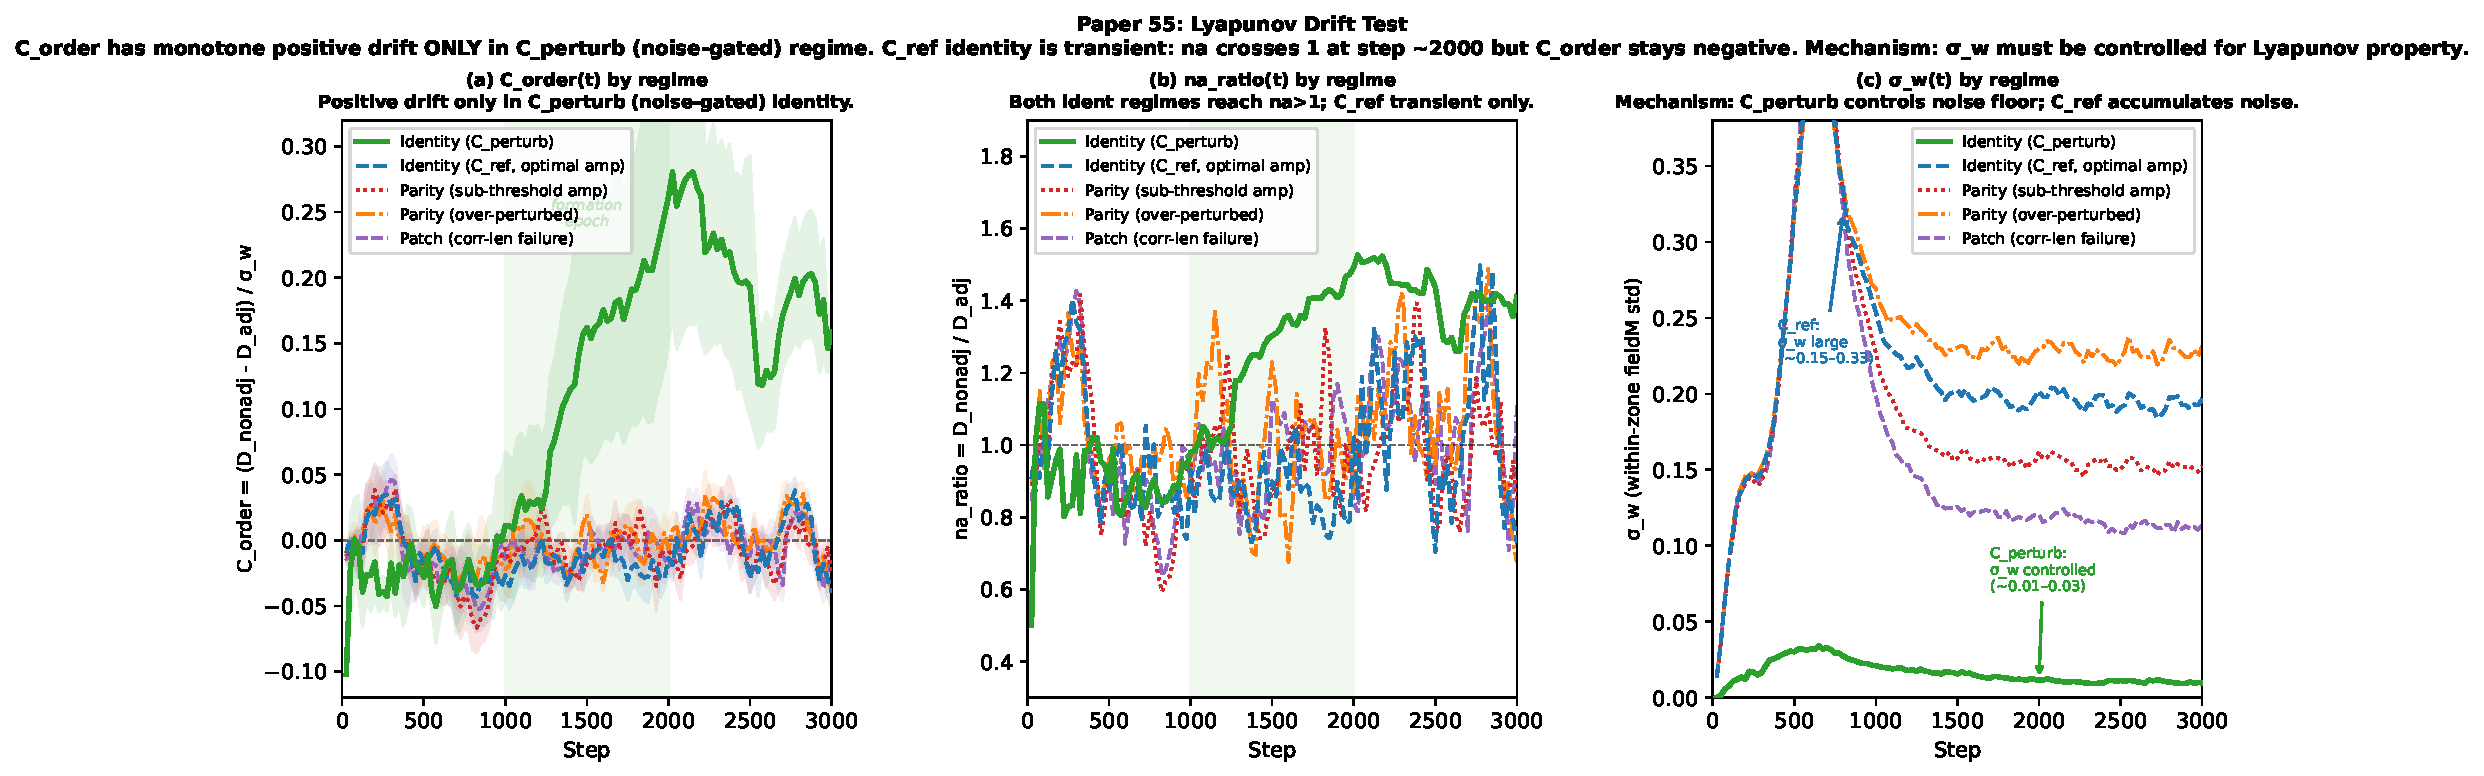
\includegraphics[width=\textwidth]{paper55_figure1.pdf}
  \caption{Three-panel Lyapunov drift test.
  (a)~C\_order(t) trajectories for five regimes.
  Only \texttt{ident\_cp} (C\_perturb, green solid) achieves positive C\_order
  with monotone drift during the formation epoch (green shaded band, steps~1000--2000).
  All C\_ref conditions remain near zero or negative.
  (b)~na\_ratio(t): both identity regimes reach na $> 1$ transiently at
  step~$\approx$2000, but only \texttt{ident\_cp} sustains it.
  (c)~$\sigma_w(t)$: the $10\times$--$20\times$ noise-floor separation between
  C\_perturb and C\_ref appears by step~500 and is maintained,
  explaining the C\_order divergence.}
\end{figure}

\end{document}
